% Options for packages loaded elsewhere
\PassOptionsToPackage{unicode}{hyperref}
\PassOptionsToPackage{hyphens}{url}
%
\documentclass[
]{article}
\usepackage{amsmath,amssymb}
\usepackage{lmodern}
\usepackage{iftex}
\ifPDFTeX
  \usepackage[T1]{fontenc}
  \usepackage[utf8]{inputenc}
  \usepackage{textcomp} % provide euro and other symbols
\else % if luatex or xetex
  \usepackage{unicode-math}
  \defaultfontfeatures{Scale=MatchLowercase}
  \defaultfontfeatures[\rmfamily]{Ligatures=TeX,Scale=1}
\fi
% Use upquote if available, for straight quotes in verbatim environments
\IfFileExists{upquote.sty}{\usepackage{upquote}}{}
\IfFileExists{microtype.sty}{% use microtype if available
  \usepackage[]{microtype}
  \UseMicrotypeSet[protrusion]{basicmath} % disable protrusion for tt fonts
}{}
\makeatletter
\@ifundefined{KOMAClassName}{% if non-KOMA class
  \IfFileExists{parskip.sty}{%
    \usepackage{parskip}
  }{% else
    \setlength{\parindent}{0pt}
    \setlength{\parskip}{6pt plus 2pt minus 1pt}}
}{% if KOMA class
  \KOMAoptions{parskip=half}}
\makeatother
\usepackage{xcolor}
\usepackage[margin=1in]{geometry}
\usepackage{graphicx}
\makeatletter
\def\maxwidth{\ifdim\Gin@nat@width>\linewidth\linewidth\else\Gin@nat@width\fi}
\def\maxheight{\ifdim\Gin@nat@height>\textheight\textheight\else\Gin@nat@height\fi}
\makeatother
% Scale images if necessary, so that they will not overflow the page
% margins by default, and it is still possible to overwrite the defaults
% using explicit options in \includegraphics[width, height, ...]{}
\setkeys{Gin}{width=\maxwidth,height=\maxheight,keepaspectratio}
% Set default figure placement to htbp
\makeatletter
\def\fps@figure{htbp}
\makeatother
\setlength{\emergencystretch}{3em} % prevent overfull lines
\providecommand{\tightlist}{%
  \setlength{\itemsep}{0pt}\setlength{\parskip}{0pt}}
\setcounter{secnumdepth}{-\maxdimen} % remove section numbering
\usepackage{booktabs}
\usepackage{longtable}
\usepackage{array}
\usepackage{multirow}
\usepackage{wrapfig}
\usepackage{float}
\usepackage{colortbl}
\usepackage{pdflscape}
\usepackage{tabu}
\usepackage{threeparttable}
\usepackage{threeparttablex}
\usepackage[normalem]{ulem}
\usepackage{makecell}
\usepackage{xcolor}
\ifLuaTeX
  \usepackage{selnolig}  % disable illegal ligatures
\fi
\IfFileExists{bookmark.sty}{\usepackage{bookmark}}{\usepackage{hyperref}}
\IfFileExists{xurl.sty}{\usepackage{xurl}}{} % add URL line breaks if available
\urlstyle{same} % disable monospaced font for URLs
\hypersetup{
  pdftitle={Mercado de Trabalho no Setor Portuário brasileiro e maranhense},
  pdfauthor={Observatório Portuário},
  hidelinks,
  pdfcreator={LaTeX via pandoc}}

\title{Mercado de Trabalho no Setor Portuário brasileiro e maranhense}
\author{Observatório Portuário}
\date{}

\begin{document}
\maketitle

{
\setcounter{tocdepth}{2}
\tableofcontents
}
\hypertarget{introduuxe7uxe3o}{%
\section{Introdução}\label{introduuxe7uxe3o}}

O setor portuário brasileiro impacta direta e indiretamente os destinos
e a economia do país.

O Observatório Portuário apresenta neste relatório uma síntese da
evolução do Trabalho Portuário e aquaviário no Brasil e no Maranhão.

Trata-se de um setor abrangente e com atividades diversas como
instalações portuárias, embarcações mercantes, de passageiros, pesca,
atividades em plataformas marítimas e de repação naval que movimentam
inúmeras cadeias produtivas e setores econômicos.

Espera-se que as ss informações apresentadas (a metodologia está
disponível na última seção) possam auxiliar o debate no setor e
subsidiar a elaboração de políticas de gestão públicas e privadas.

Este é o primeiro de uma série de quatro relatórios sobre o mercado de
trabalho portuário e aguaviário brasileiro e maranhense.

Boa leitura.

\hypertarget{panorama-do-trabalho-no-setor-portuuxe1rio-e-aquaviuxe1rio-no-brasil}{%
\section{Panorama do trabalho no setor portuário e aquaviário no
Brasil}\label{panorama-do-trabalho-no-setor-portuuxe1rio-e-aquaviuxe1rio-no-brasil}}

Foram 76.350 vínculos registrados no setor portuário e aquaviário no
Brasil em 2020, de acordo com os dados da Relação Anual de Informações
Sociais (RAIS).

O número apresenta um decréscimo em relação aos anos anteriores,
sobretudo em relação ano de 2018, quando quase 80 mil vínculos foram
registrados. Considerando a tendência de queda do número de vínculos
identificada a partir de 2014, reitera-se a associação entre desempenho
das atividades econômicas do país e sua influência no estoque de
empregos do setor.

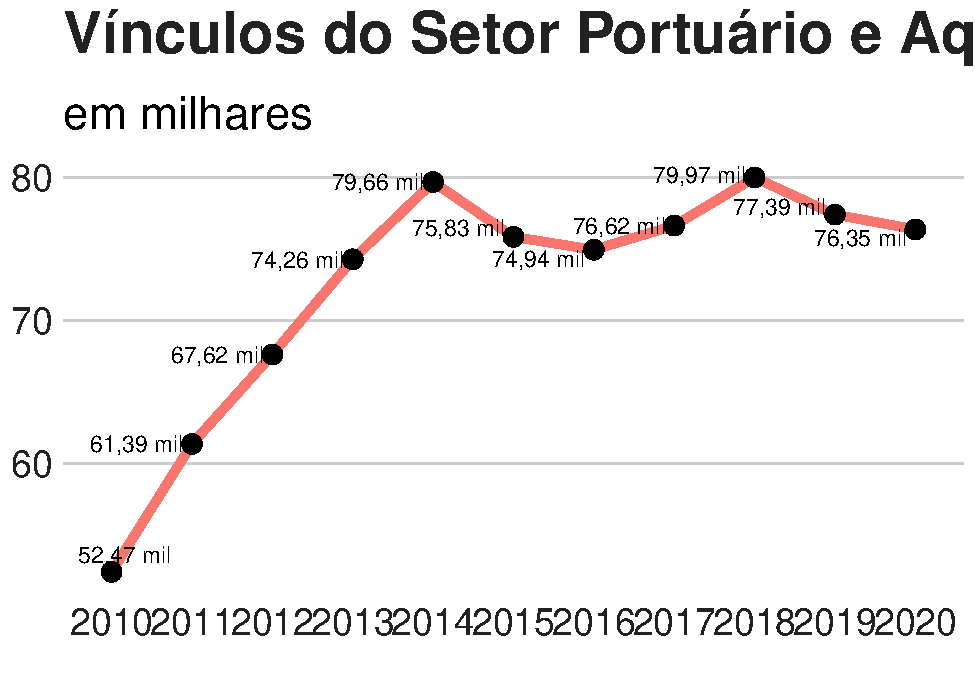
\includegraphics{mercado_trabalho_files/figure-latex/g_secao-1.pdf}

Ao analisar os dados por setor de atividade no contexto nacional,
verifica-se redução do número de vínculos no grupo de profissionais
atuantes no \textbf{Transporte aquaviário}, com uma redução de 44.420
mil vínculos em 2013 para 37.910 mil em 2020, com uma redução de 6.510
vínculos.

Por outro lado, nota-se que o grupo de atividades agrupadas como
\textbf{Armazenamento e Atividades Auxiliares dos Transportes}
apresentou um comportamento crescente no período, superando em 2020 o
número de vínculos no \textbf{Transporte aquaviário}.

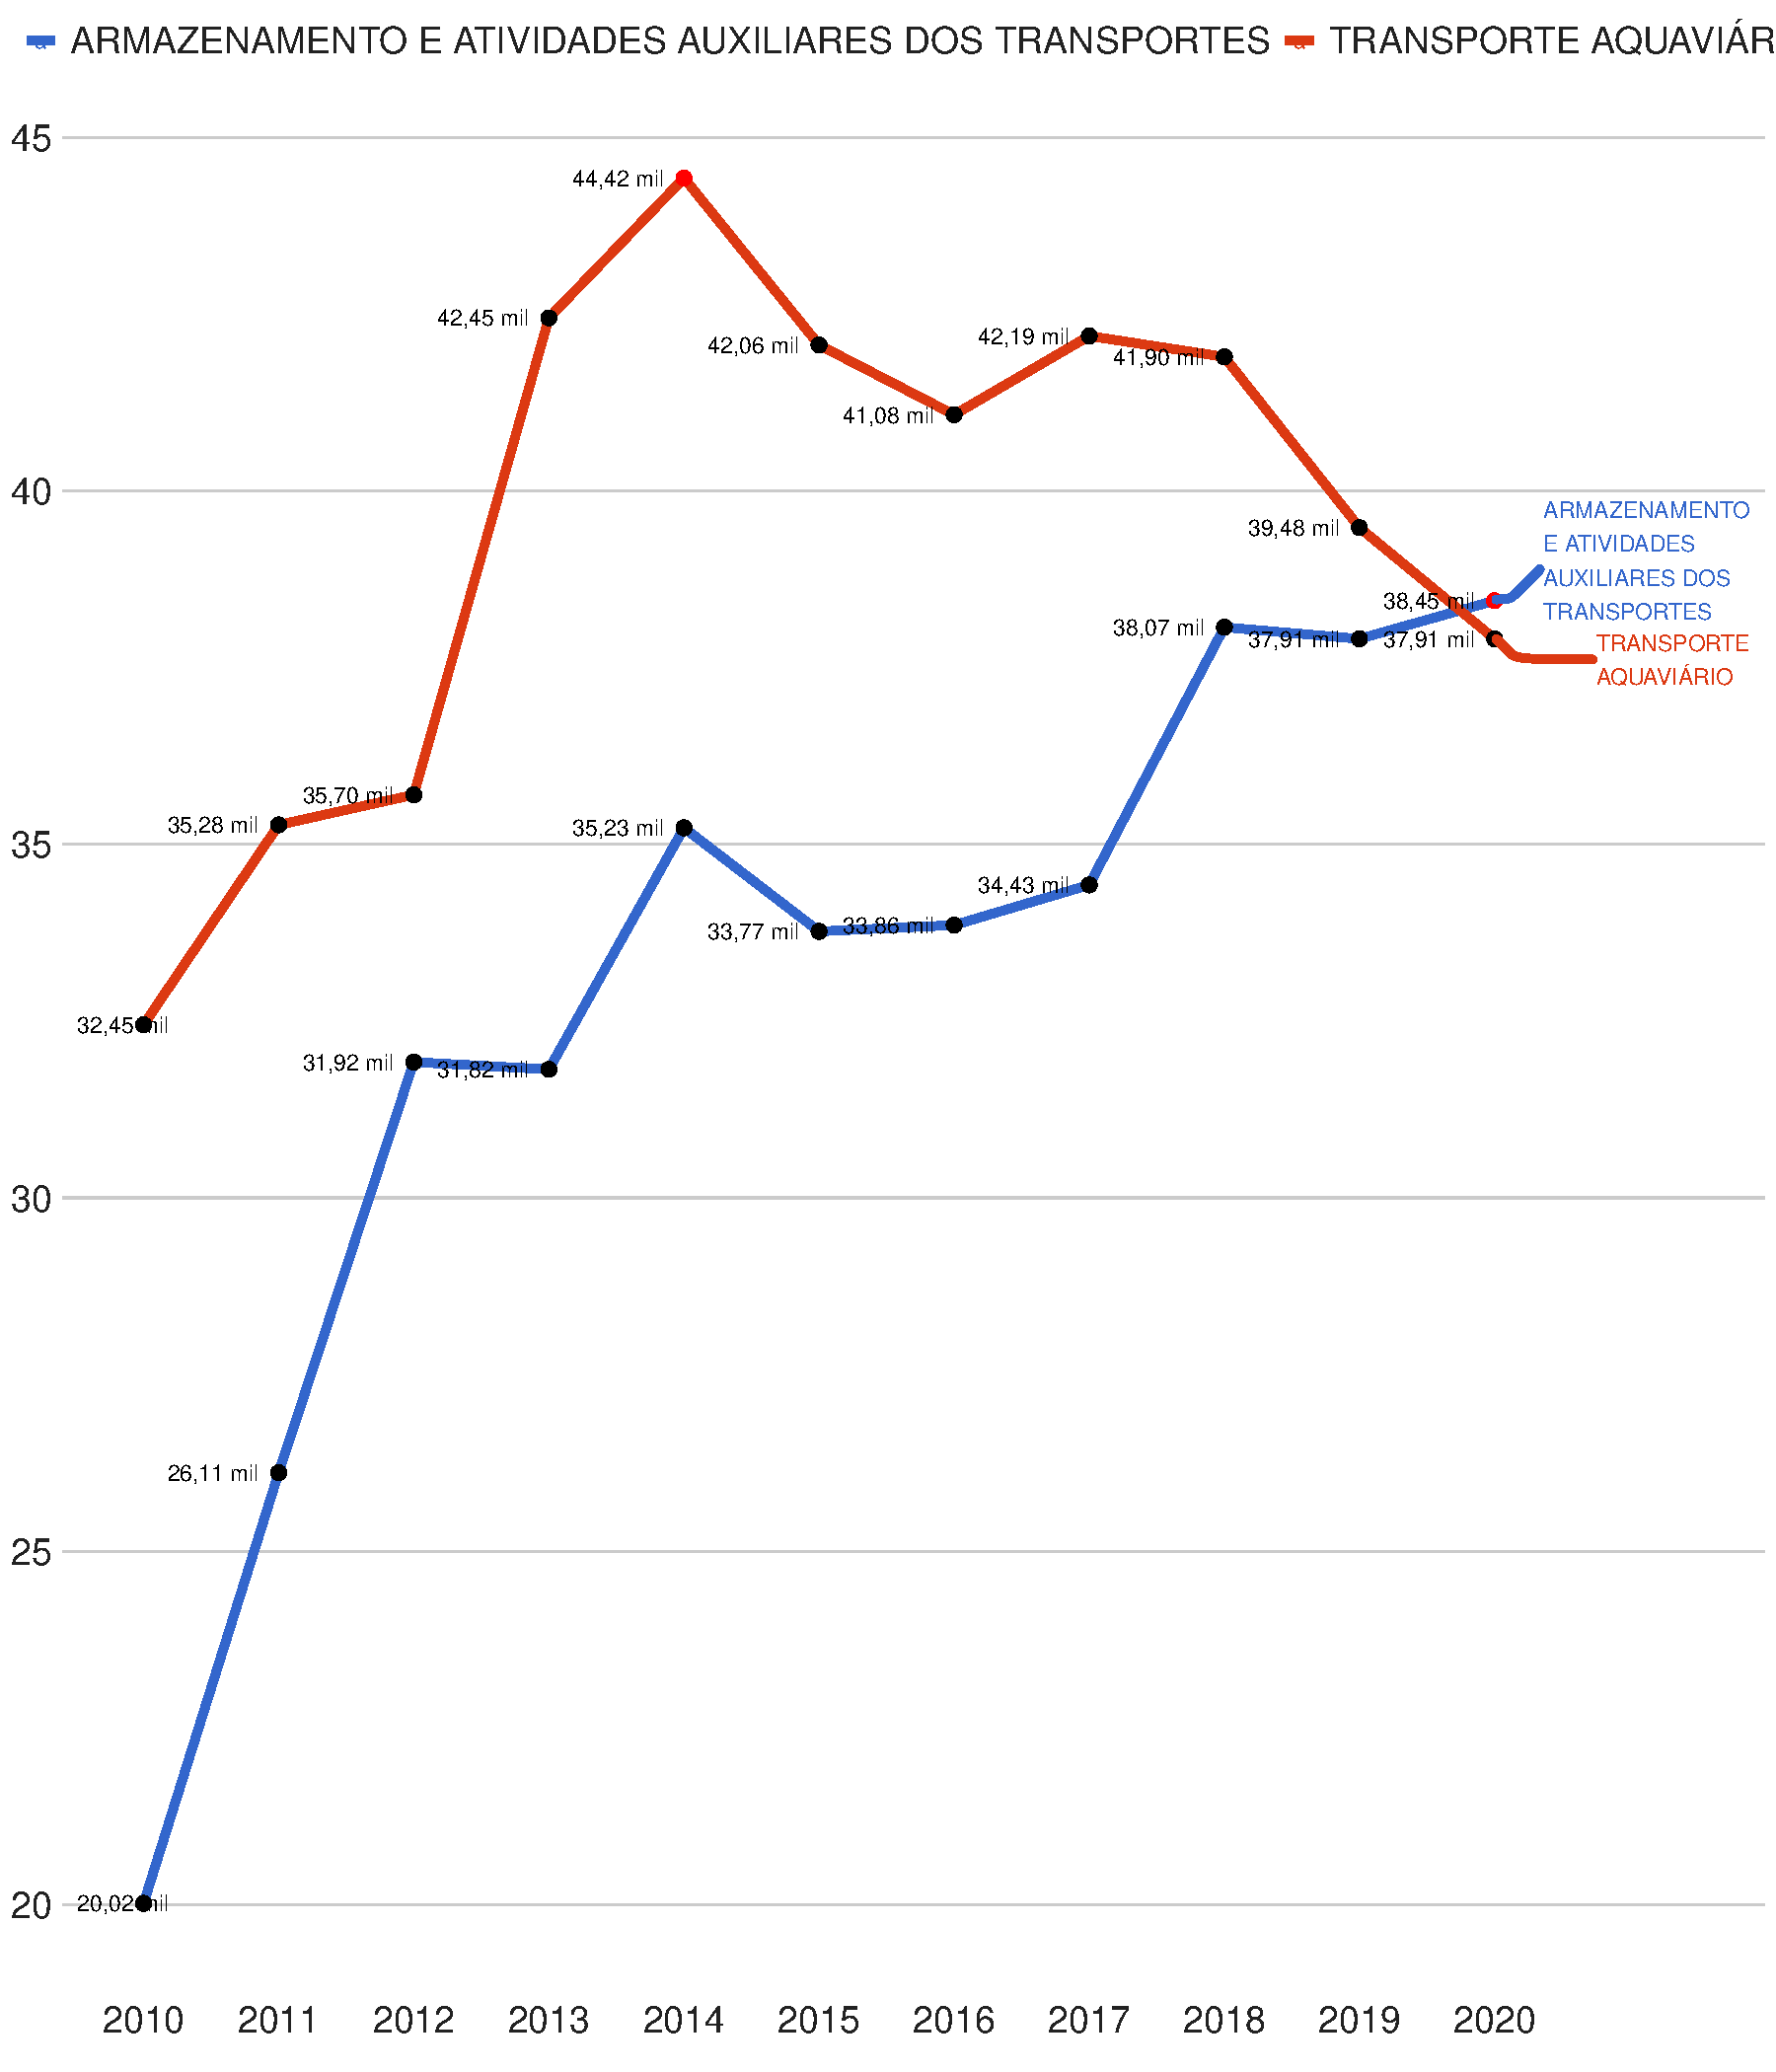
\includegraphics{mercado_trabalho_files/figure-latex/g_divisao-1.pdf}

Ao analisar os grupos de atividades com maior participação no número de
vínculos empregatícios, destacam-se as atividades de
\textbf{Armazenamento e Atividades Auxiliares dos Transportes} e
\textbf{Transporte Aguaviário}.

O \textbf{Armazenamento e Atividades Auxiliares dos Transportes}
compreende, de acordo com a Classificação Nacional de Atividades
Econômicas-CNAE, atividades relacionadas

\begin{quote}
{[}\ldots{]} com a movimentação e o armazenamento de cargas, antes ou
depois de seu transporte, ou entre segmentos de transporte de distintas
modalidades, as atividades auxiliares das diversas modalidades de
transporte envolvendo a operação da infraestrutura de suporte nas
rodovias, ferrovias, aeroportos, portos, pontes túneis, etc. e as
atividades de agenciamento de transporte. Esta divisão compreende também
as atividades relacionadas à organização do transporte de carga.
\end{quote}

Destaque também deve ser dado para o número de vínculos ``Transporte
Aguaviário**, cujas atividades são as relacionadas aos transportes de
pessoas e mercadorias, além das embarcações turísticas e o fretamento de
embarcações com tripulação. Nela também estão as operações e embarcações
para apoio marítimo e portuário.

No gráfico a seguir estão detalhados os vínculos e atividades
contemplados no Transporte Aguaviário no país.

Com o recorte, verifica-se que as atividades de \textbf{Navegação de
Apoio} apresentam o maior número de vínculo, registrando o maior número
de vínculos em 2020 na categoria (18.237). A categoria abarca atividades
como:

\begin{itemize}
\item
  o transporte de mercadorias e pessoas para suprimento e apoio a navios
  e a plataformas de pesquisas e exploração de minerais e
  hidrocarbonetos;
\item
  a navegação realizada para apoio logístico a navios e a plataformas de
  exploração de minerais e hidrocarbonetos transporte;
\item
  a navegação realizada nos portos e terminais aquaviários, para
  atendimento a embarcações e instalações portuárias;
\item
  os serviços de reboque realizado por empresas de apoio marítimo;
\item
  os serviços de socorro e salvamento realizado por empresas de apoio
  portuário.
\end{itemize}

Observa-se que o grupo de \textbf{Transporte por Navegação Interior},
segundo maior grupo em número de vínculos no \textbf{Transporte
Aguaviário}, finalizou 2020 com 11.488 vínculos. São atividades como
\emph{o transporte de carga municipal, por rios, canais, lagos, lagoas,
baias e outras vias de navegação interior, exceto travessia} e \emph{o
fretamento de embarcações com tripulação}, mas não inclui a
\emph{operação e gestão de terminais de carga}.

\hfill\break

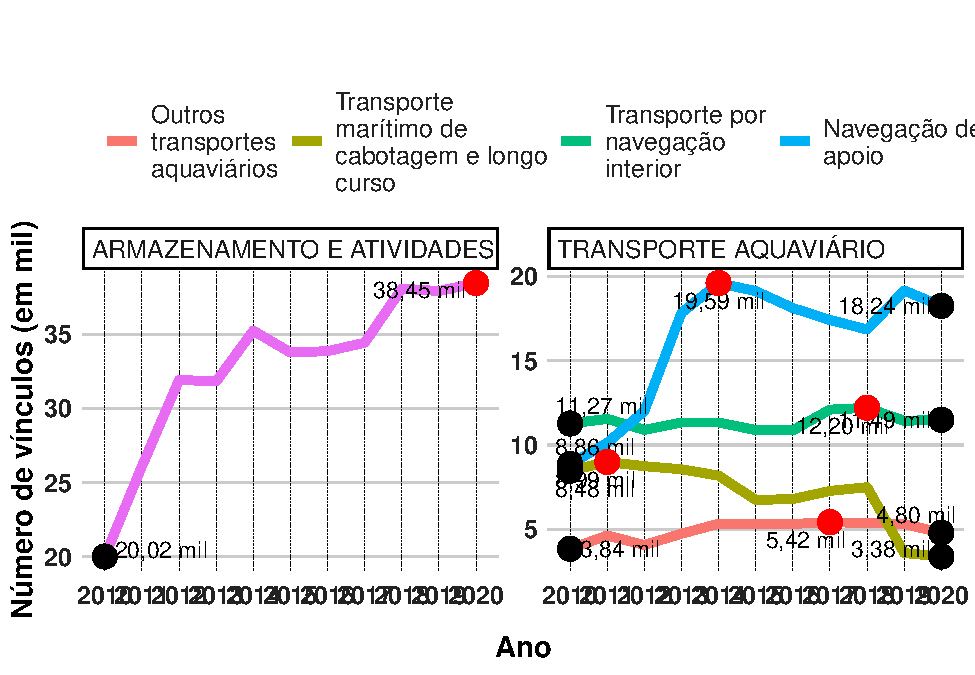
\includegraphics{mercado_trabalho_files/figure-latex/g_grupo-1.pdf}

Esses dados podem detalhados um pouco mais a partir da análise das
seções da Classificação Nacional de Atividades Econômicas (CNAE) do
Instituto Brasileiro de Geografia e Estatística (IBGE), o que permite
identificar quais áreas impactaram diretamente o estoque de empregos na
área portuária e aguaviária.

Pelo gráfico a seguir, alguns destaques do setor podem ser obtidos por
grupo de atividade:

\begin{itemize}
\item
  Ao considerar a \textbf{Gestão de Portos e Terminais}, o destaque foi
  para as \emph{Operações de Terminais}, que apresentou número crescente
  de vínculos entre 2010 e 2020, registrando 35.357 vínculos. Por outro
  lado, as atividades de Administração da Infra-estrutura Portuária
  tiveram um declínio de 41,25\%, resultado da destruição de 2.170
  vínculos;
\item
  O \textbf{Transporte Marítico de Carga por Cabotagem}, por sua vez,
  teve uma redução drástica de vínculos: saiu de 8.289 em 2010 para
  3.316 em 2020.
\item
  O \textbf{Transporte por Navegação Interior de Carga}, por outro lado,
  apresentou leve aumento: passou de 7.524 para 8.382 vínculos.
\item
  A \textbf{Navegação de Apoio Marítimo}, por sua vez, duplicou o número
  de vínculos e chegou a 15.372 profissionais na área.
\end{itemize}

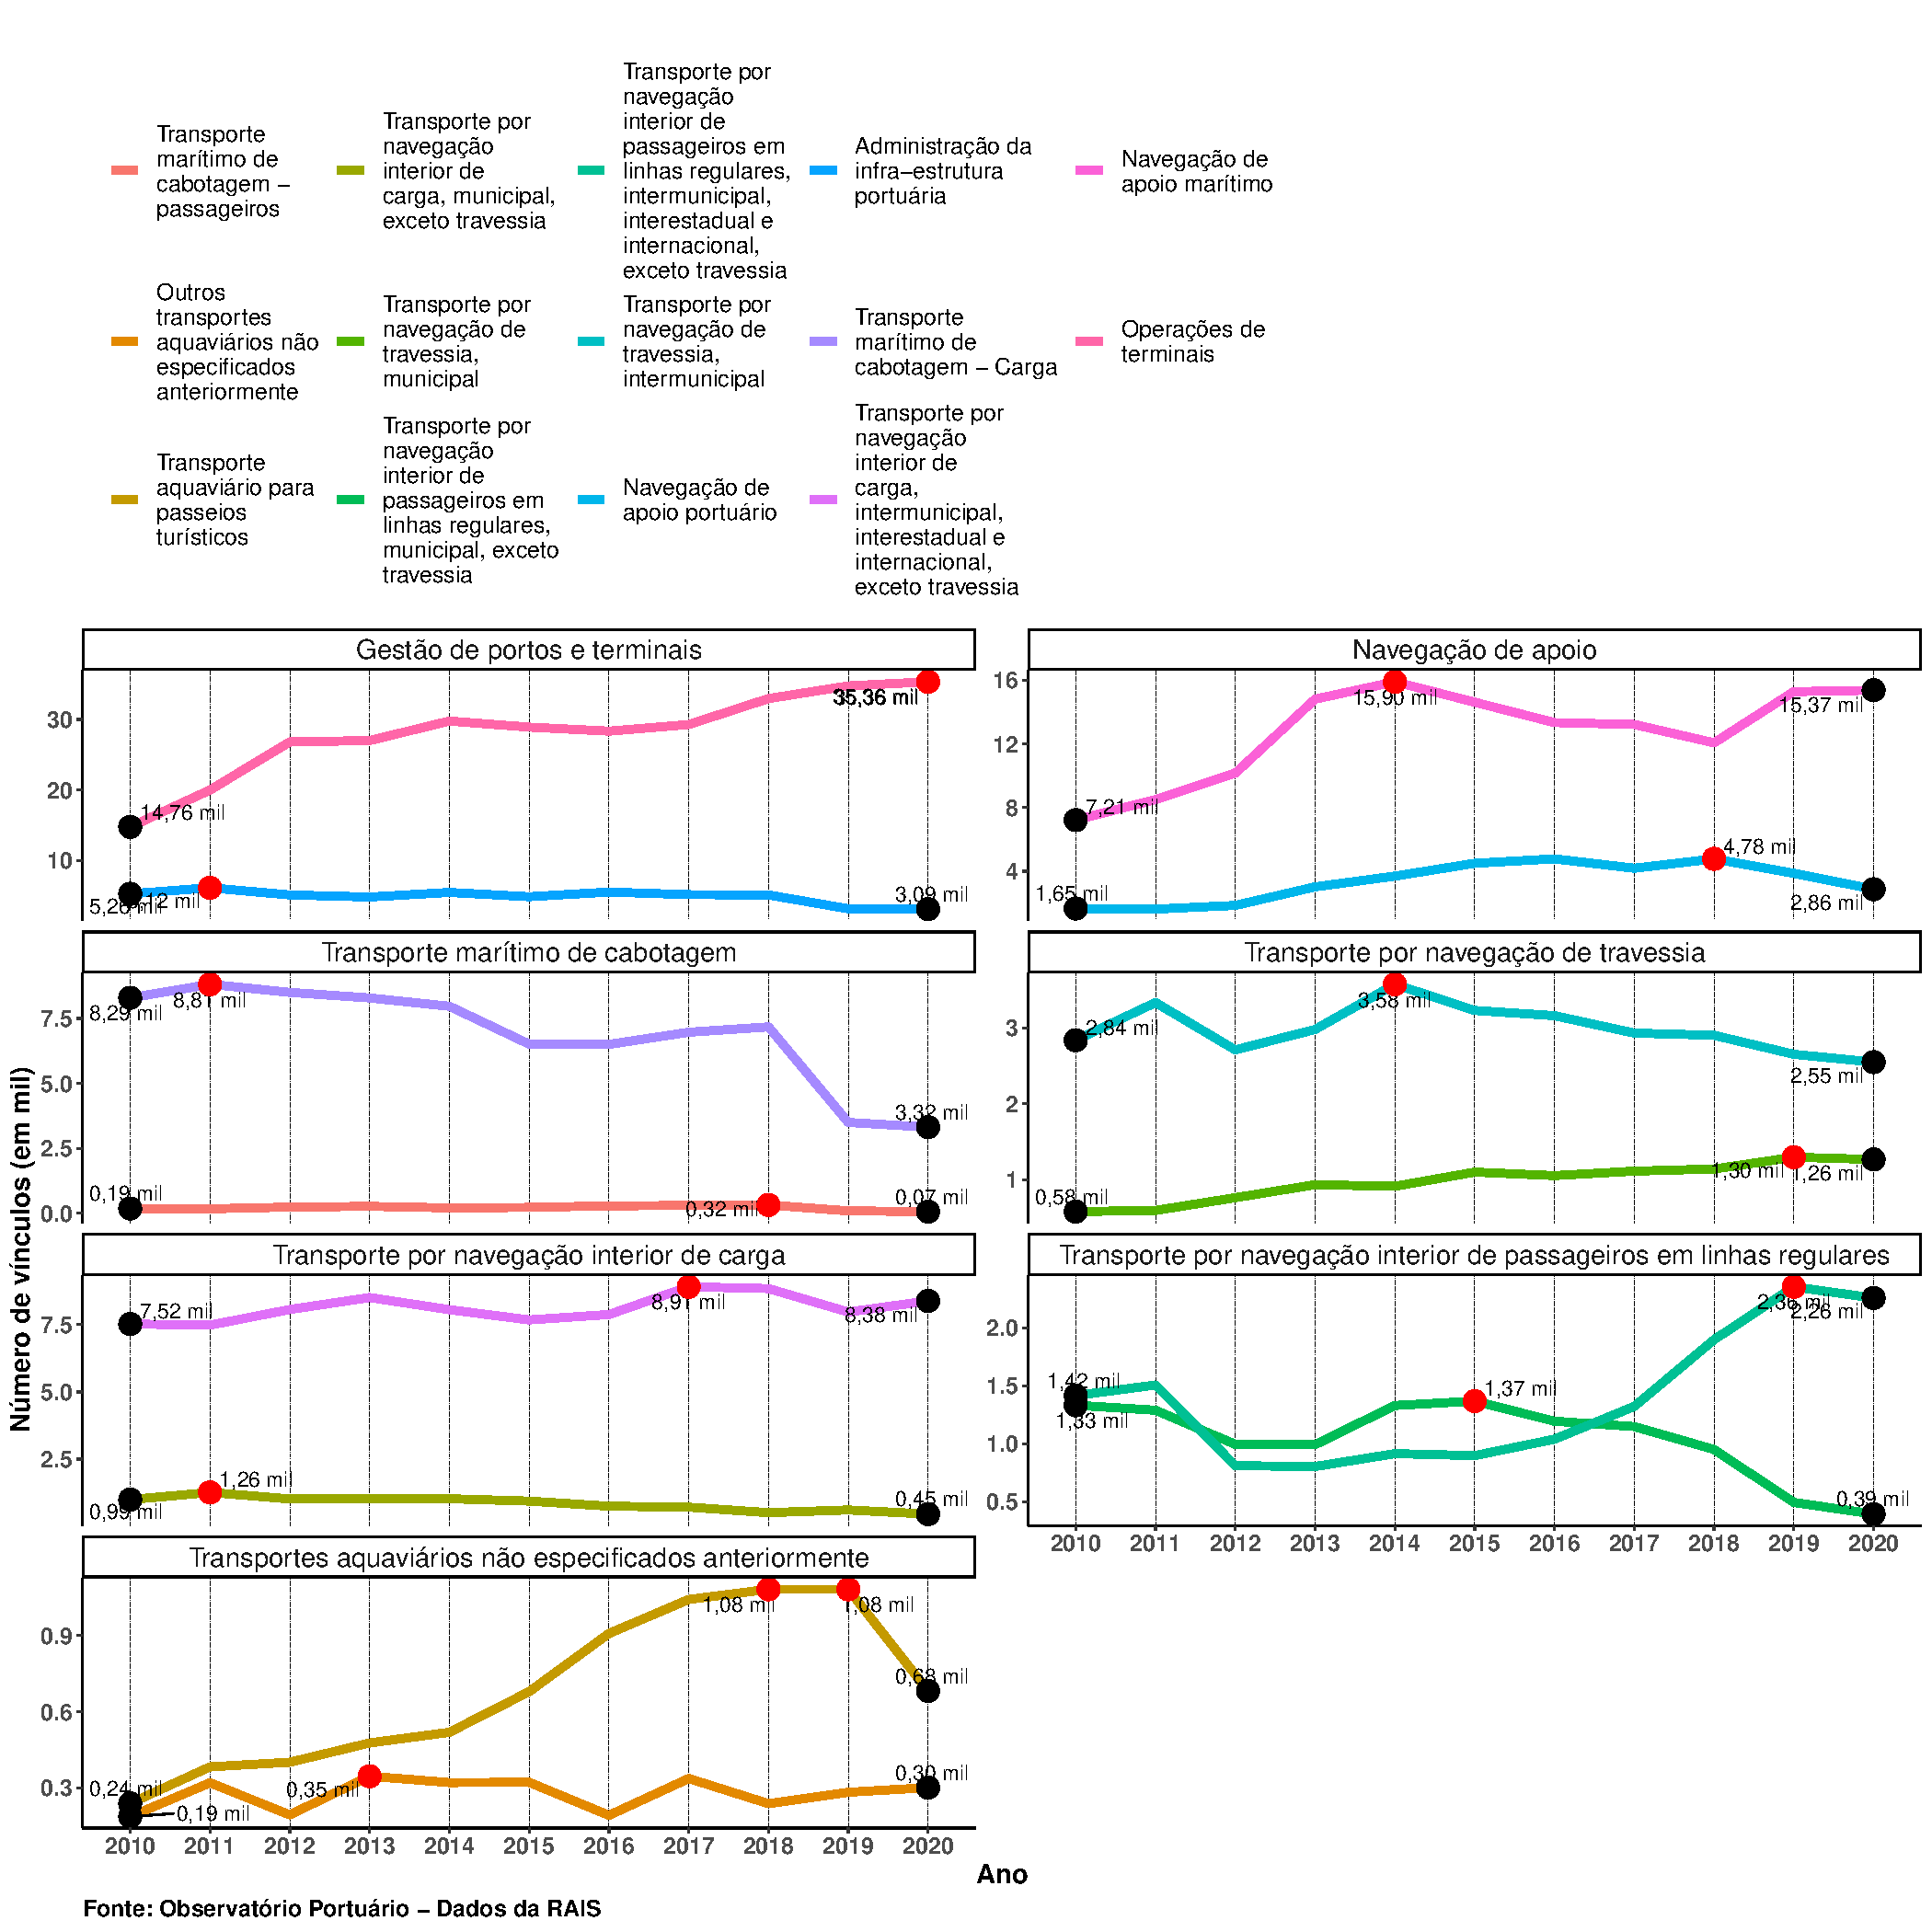
\includegraphics{mercado_trabalho_files/figure-latex/funcao2-1.pdf}

Os dados são um reflexo das políticas de regulação para o setor,
evidenciando como as estratégias governamentais e empresariais se
refletem no estoque de empregos no setor.

Na próxima seção os dados para o estado do Maranhão são apresentados.

\hypertarget{panorama-do-trabalho-no-setor-portuuxe1rio-e-aquaviuxe1rio-no-maranhuxe3o}{%
\section{Panorama do trabalho no setor portuário e aquaviário no
Maranhão}\label{panorama-do-trabalho-no-setor-portuuxe1rio-e-aquaviuxe1rio-no-maranhuxe3o}}

Ao analisar os dados para o estado do Maranhão, verifica-se que os
vínculos diretos foram ascendentes até o ano de 2017, quando foram
identificados 2.016 vínculos. Em 2020, depois de quedas em 2018 e 2019,
apresentou ligeira recuperação e o número de vínculos registrados foi de
1.924.

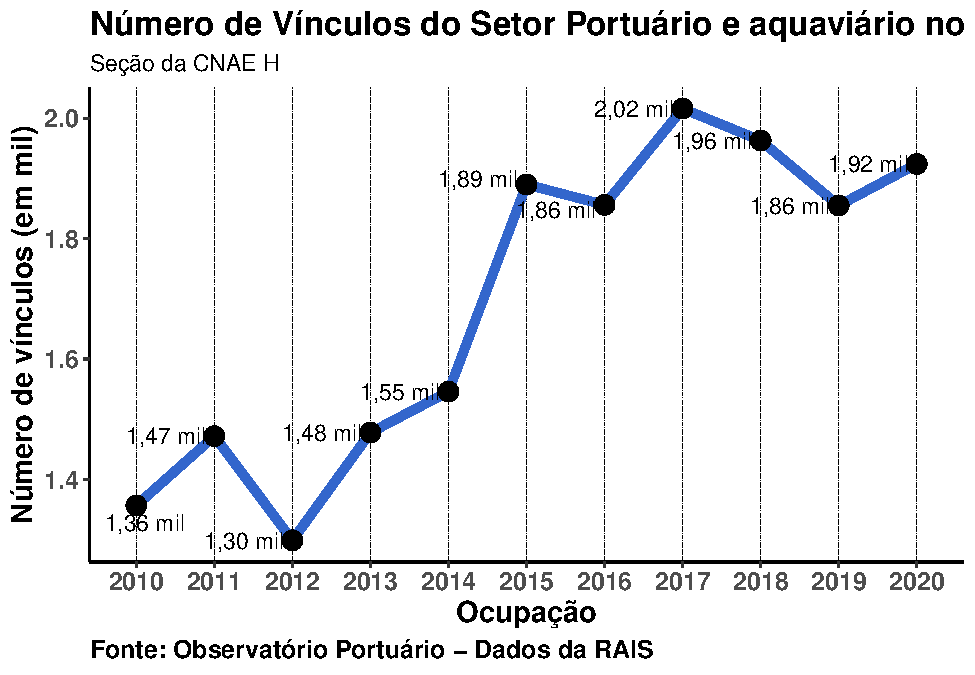
\includegraphics{mercado_trabalho_files/figure-latex/g_secao_ma-1.pdf}

No caso do Maranhão, o \textbf{Transporte Aguaviário} é o grupo de
atividade que apresenta o maior número de empregos diretos, com 1.000
vínculos em 2020.

Ao mesmo tempo, as atividades abarcadas pelo \textbf{Armazenamento e
Atividades Auxiliares dos Transportes} apresentaram permanente
crescimento no perído, o que se relaciona com o aumento das atividades
portuárias no estado,com o registro de 920 vínculos em 2020.

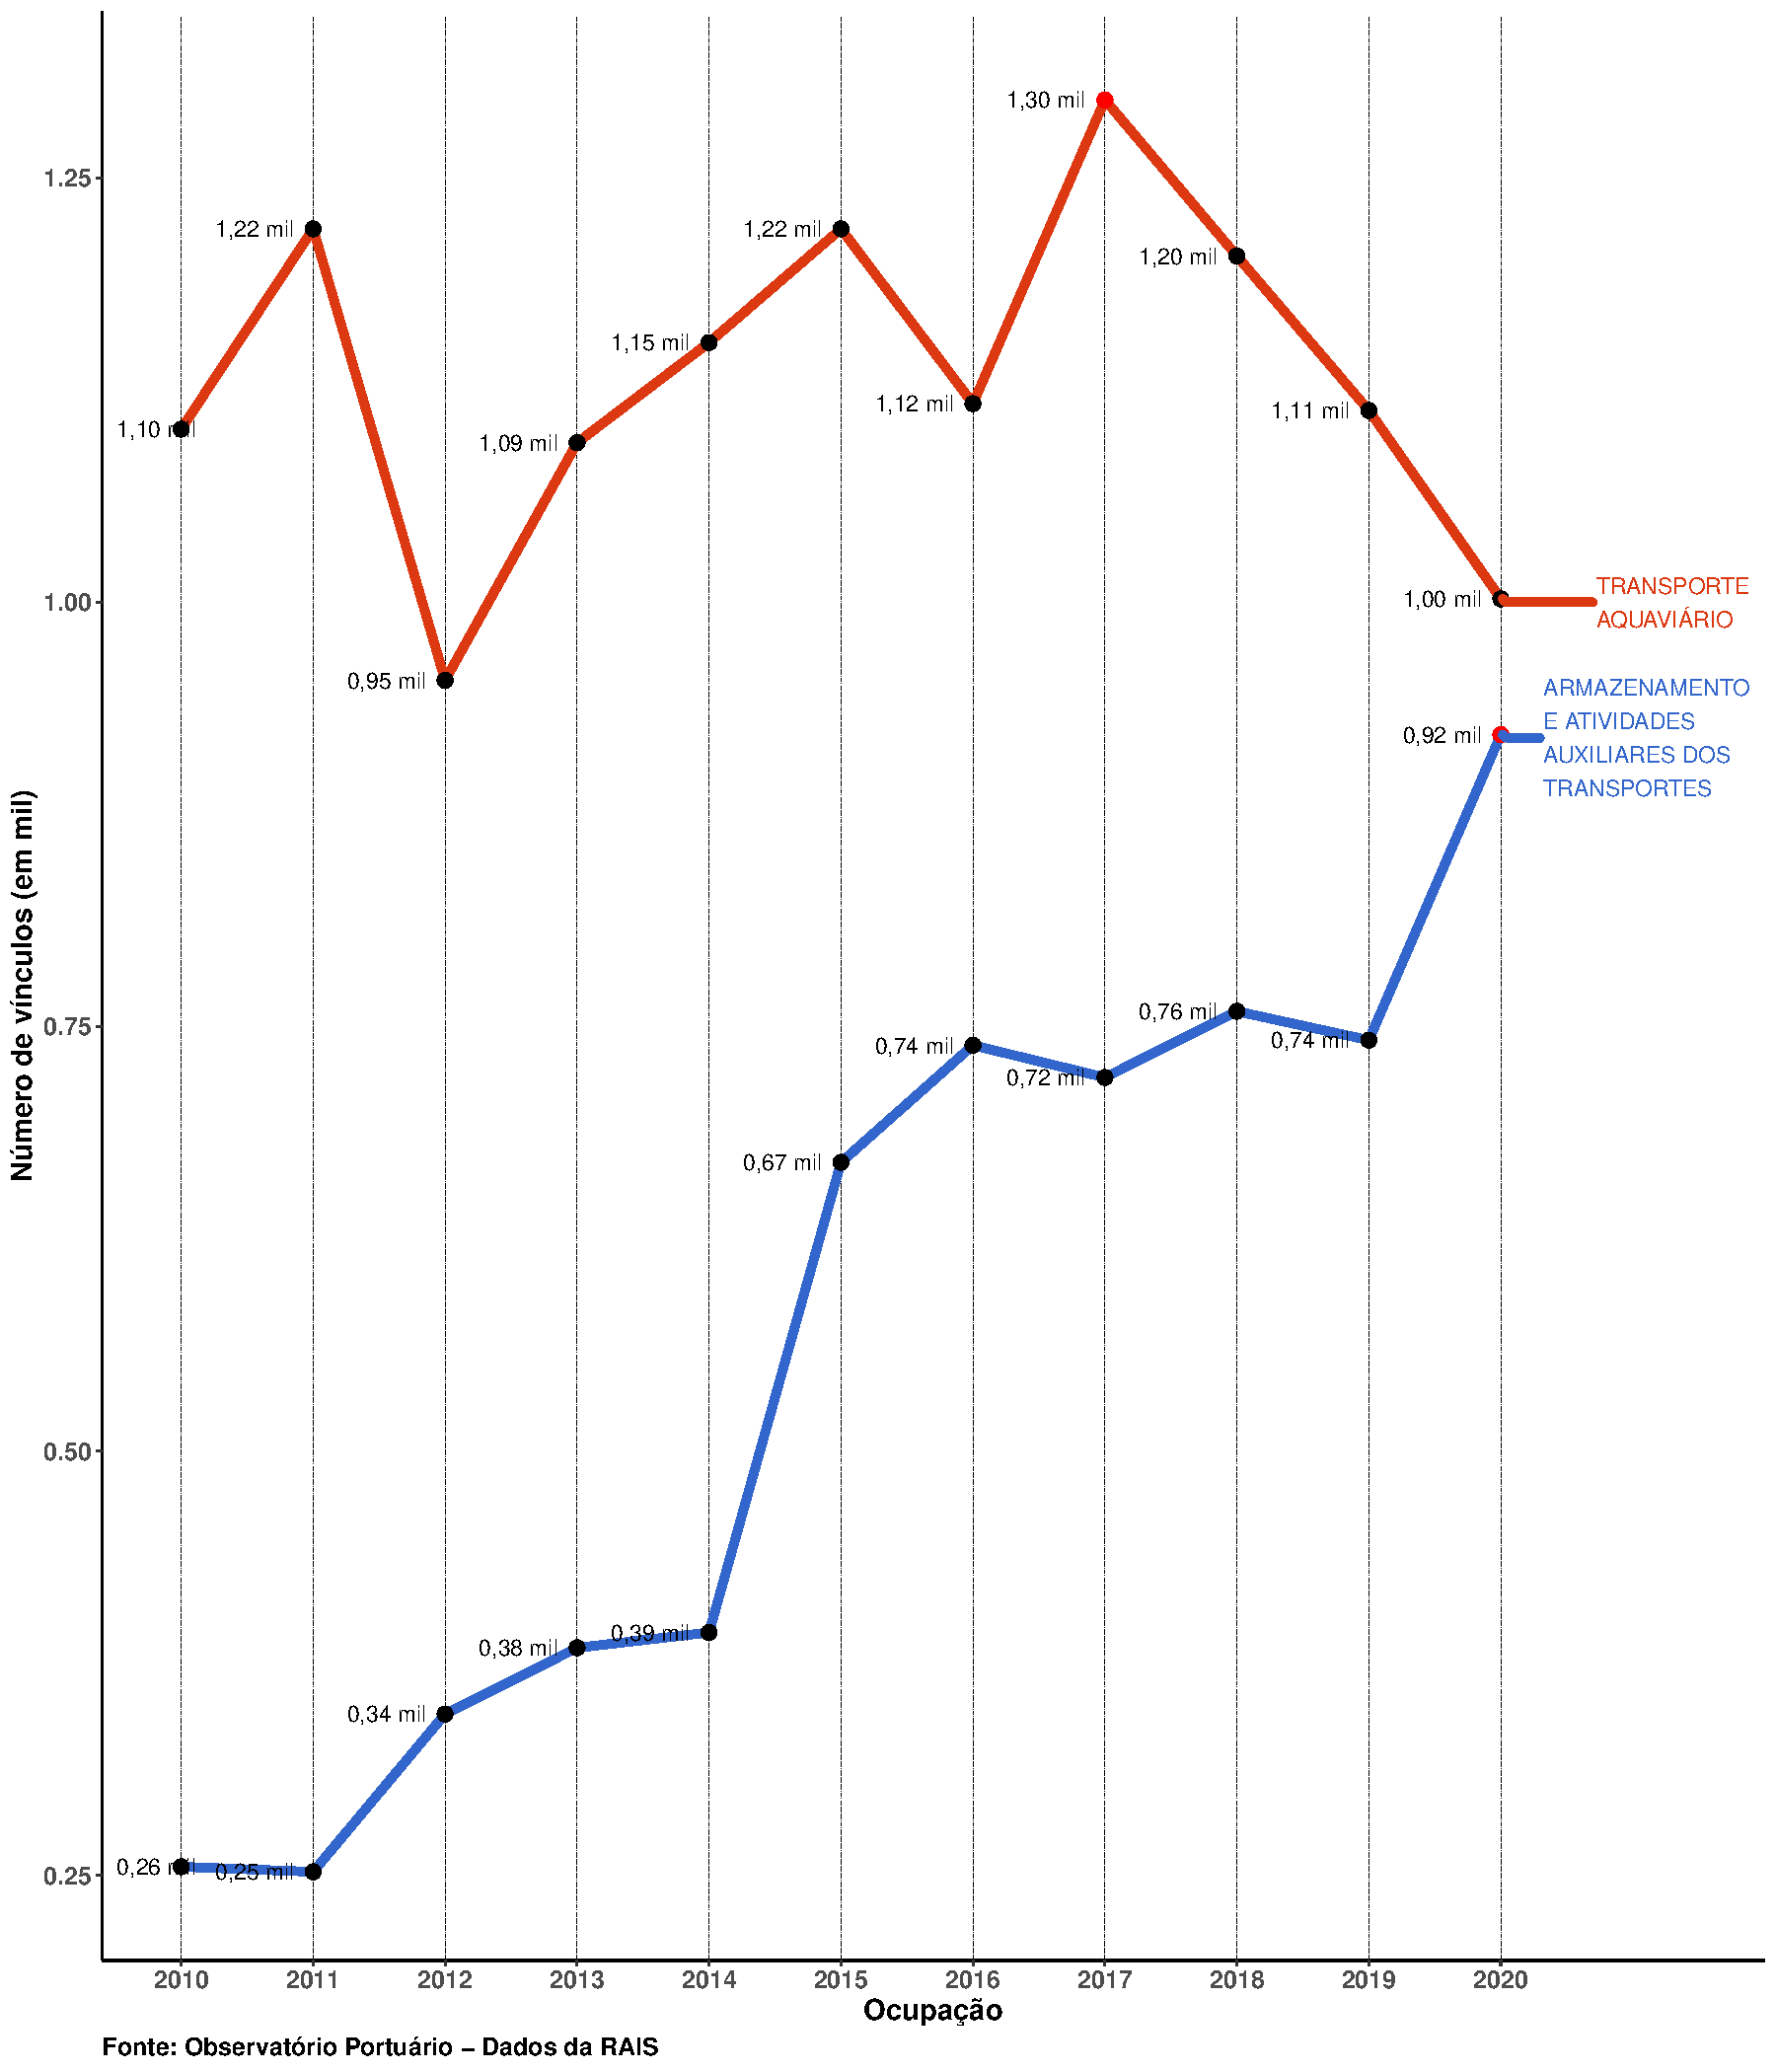
\includegraphics{mercado_trabalho_files/figure-latex/g_divisao_ma-1.pdf}

No gráfico a seguir pode-se observar as modalidades abarcadas pelo
\textbf{Transporte Aguaviário} e suas representatividades no estado. O
destaque positivo é para o setor de \textbf{Navegação de Apoio}, que
auxilia as atividades portuárias.

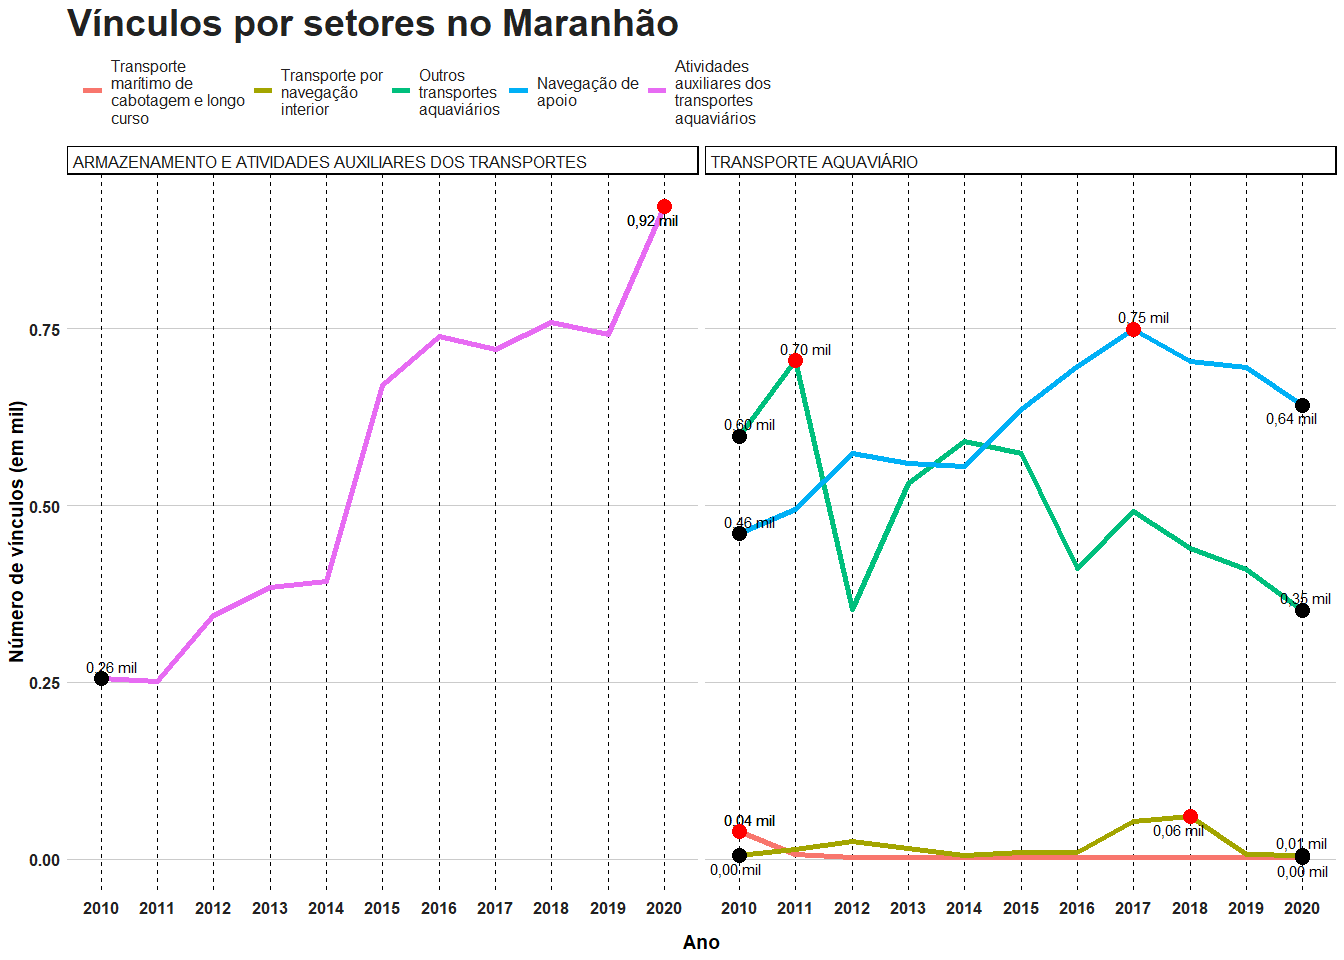
\includegraphics{mercado_trabalho_files/figure-latex/g_grupo_ma-1.pdf}

Ao analisar as subclasses de atividade, pode-se verificar que as
atividades relacionadas a \textbf{Operações de Terminais} teve excelente
resultado, saltando de 14 para 920 mil vínculos, o que indica uma
transformação estrutural nas atividades.

A \textbf{Navegação de Apoio Marítimo} e \textbf{Navegação de Apoio
Portuário} também se destacam, embora com oscilações consideráveis na
série.

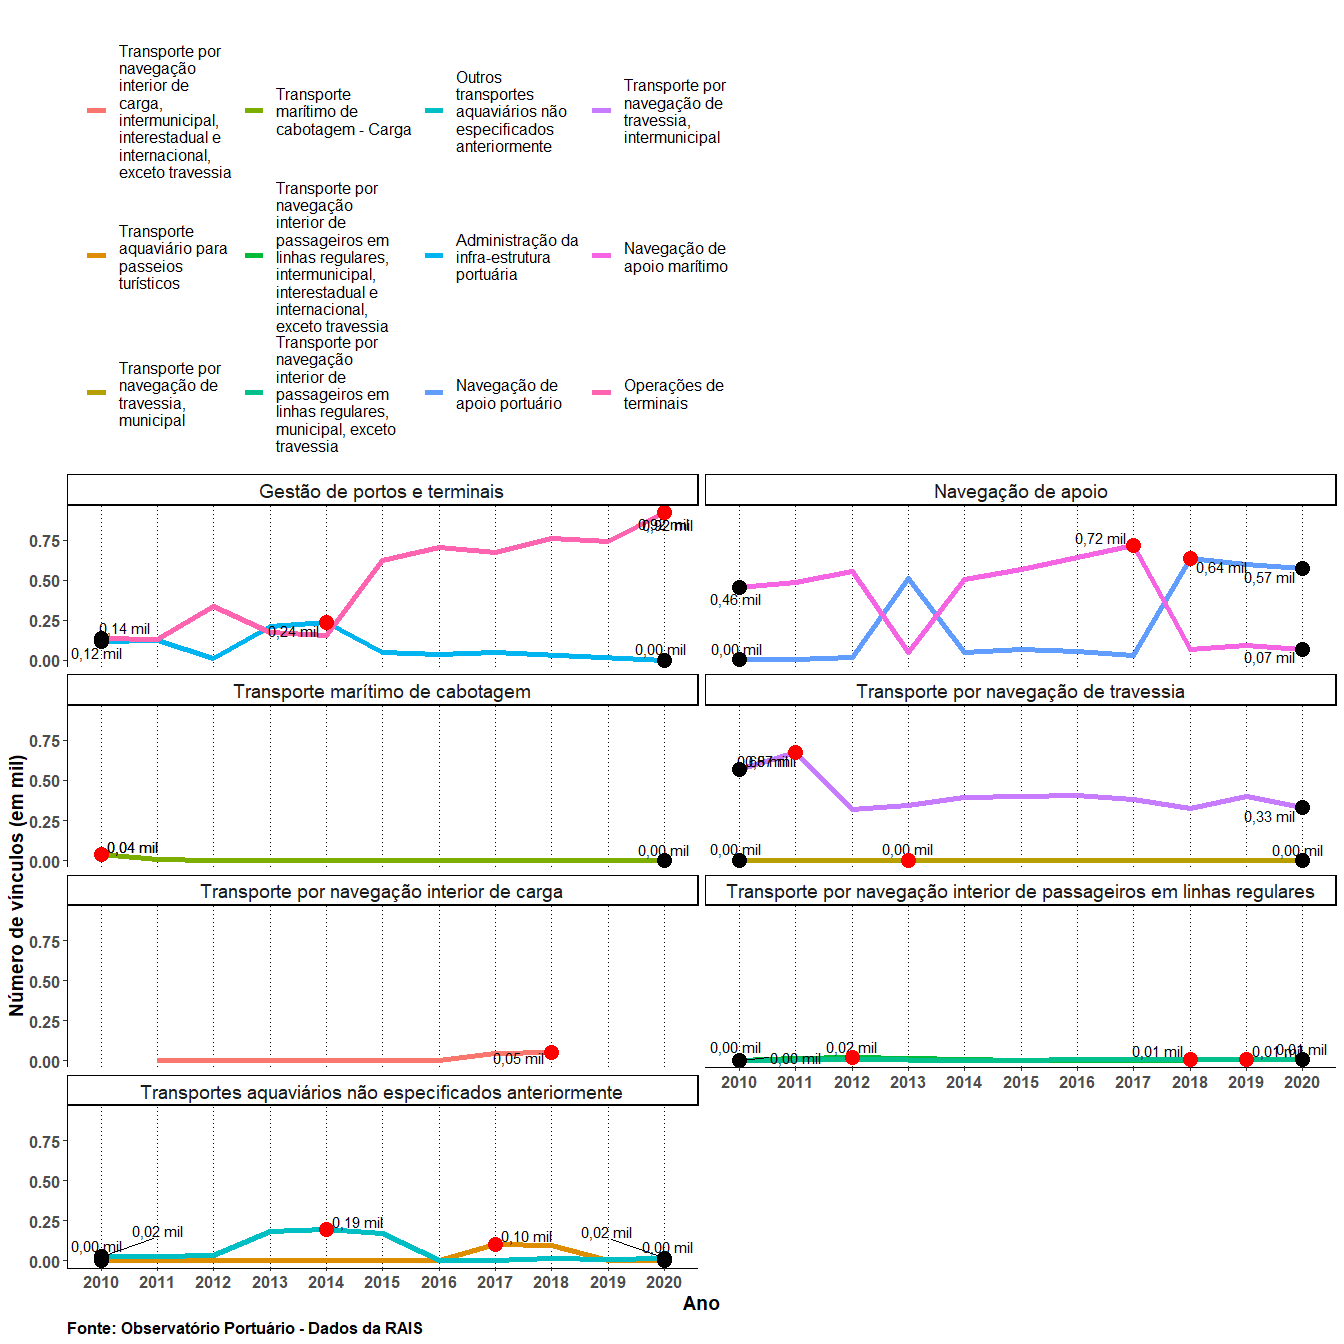
\includegraphics{mercado_trabalho_files/figure-latex/subclasse.ma-1.pdf}

\hypertarget{perfil-do-trabalhador-portuuxe1rio-e-aquaviuxe1rio}{%
\section{Perfil do Trabalhador Portuário e
Aquaviário}\label{perfil-do-trabalhador-portuuxe1rio-e-aquaviuxe1rio}}

\hypertarget{escolaridade-do-trabalhador-portuuxe1rio-e-aquaviuxe1rio}{%
\paragraph{Escolaridade do Trabalhador Portuário e
aquaviário}\label{escolaridade-do-trabalhador-portuuxe1rio-e-aquaviuxe1rio}}

Ao analisar o perfil dos trabalhadores portuários e aguaviários por
sexo, observa-se que a participação masculina é predominante. Em 2020,
do total de 76.317 vínculos, 65.735 eram homens, sendo apenas 10.582
mulheres (13,87\%).

No Maranhão a proporção é igual: dos 1.924 vínculos, apenas 14\% eram
mulheres (2.629)

Apesar da baixa participação feminina no setor, observa-se que elas
apresentavam maior escolaridade no contexto nacional: 44,5\% tinham
curso superior, contra 17,7\% dos homens com a mesma escolaridade. De
forma agregada, observa-se o aumento da escolarização entre 2010 e 2020,
apesar do número de profissionais com pós-graduação ainda ser baixo.

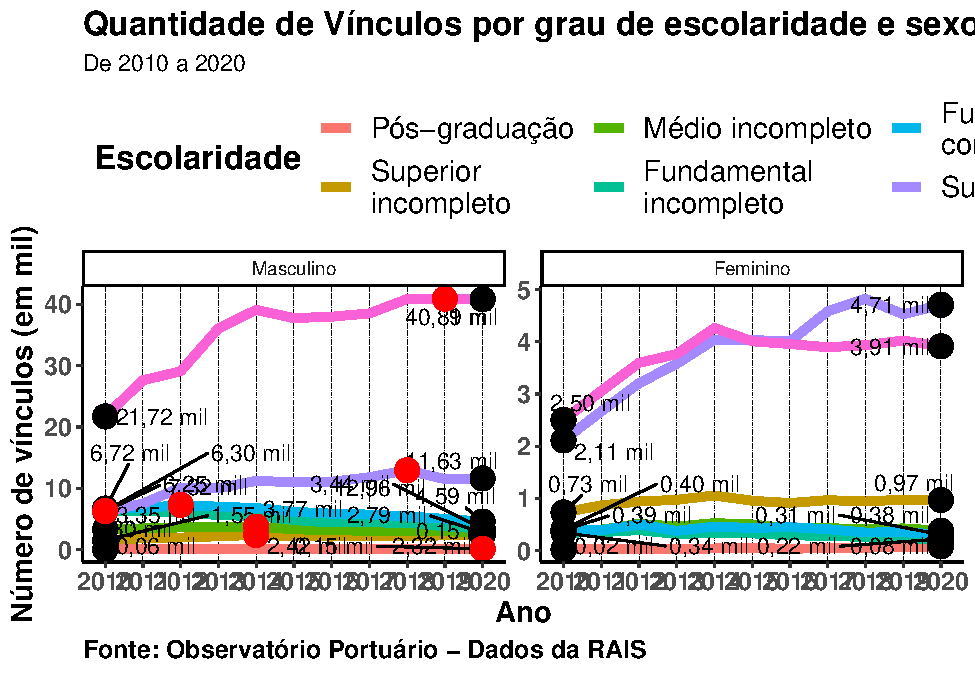
\includegraphics{mercado_trabalho_files/figure-latex/g_operacao_escol_sexo-1.pdf}

O Maranhão também acompanha a tendência nacional no quesito
escolarização: há o predomínio de profissionais com ensino médio
completo e, em seguida, ensino superior. Apesar de crescente, o número
de pessoas com pós-graduação ainda é incipiente, o que irá refletir na
remuneração, como se observa no gráfico:

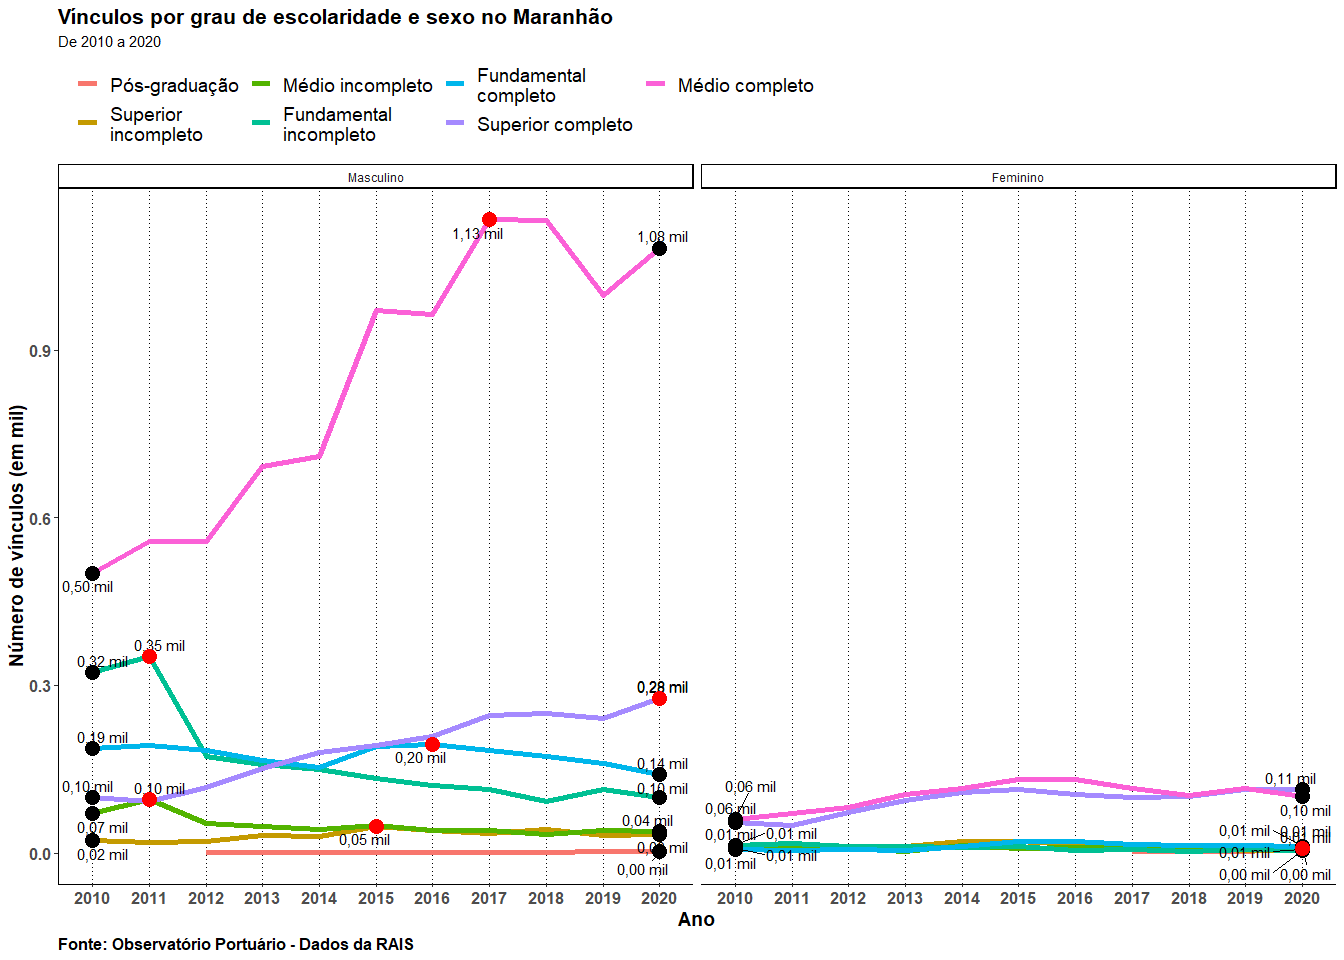
\includegraphics{mercado_trabalho_files/figure-latex/g_operacao_escol_sexo.ma-1.pdf}

Ao avaliar a remuneração média por escolaridade no país, verifica-se que
os profissionais com pós-graduação têm uma renda significativamente
superior aos demais níveis de escolaridade.

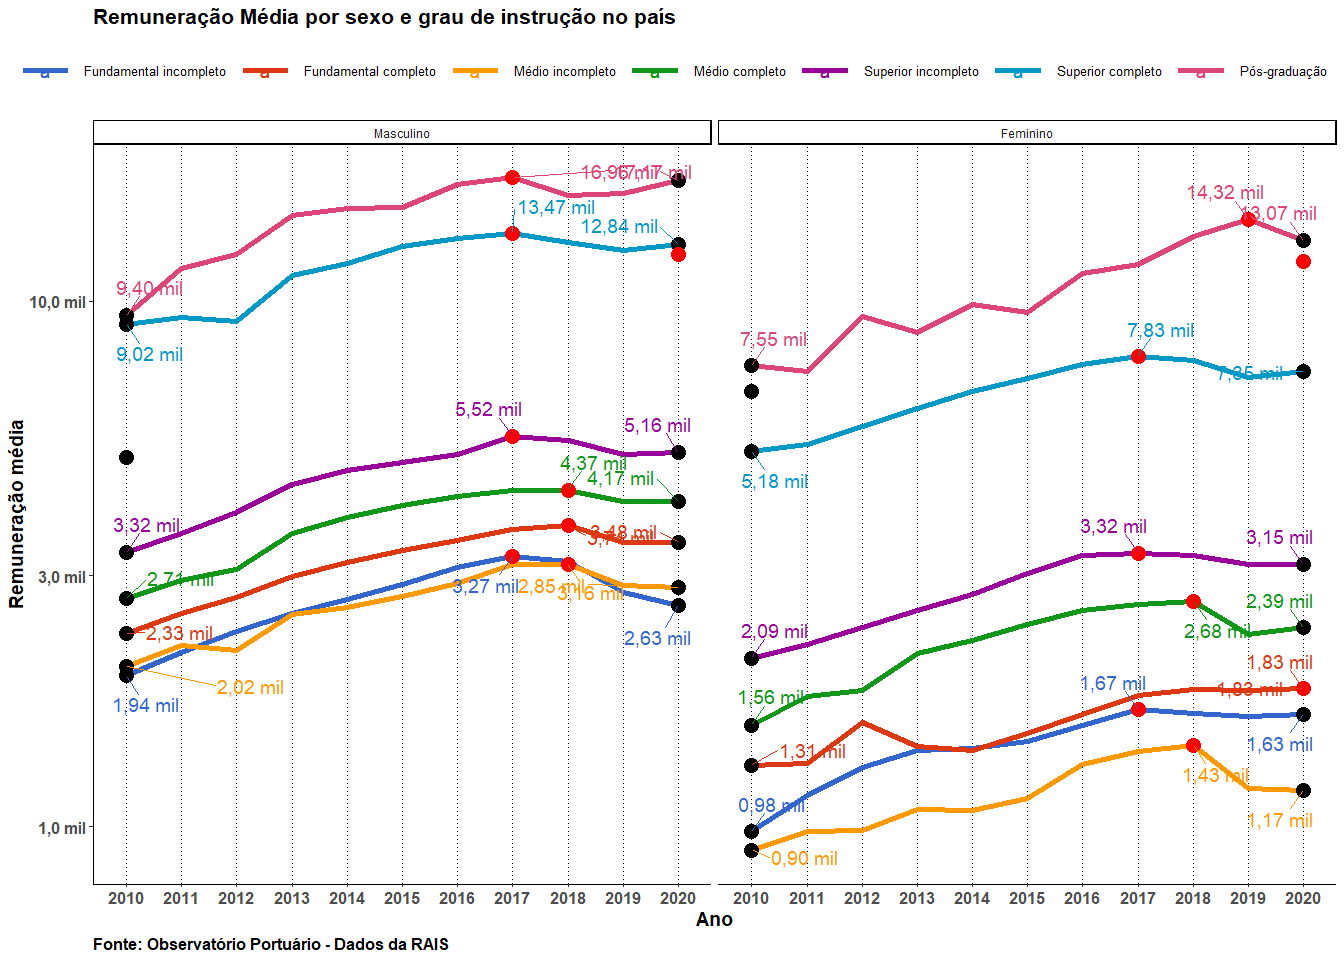
\includegraphics{mercado_trabalho_files/figure-latex/g_remun_escol_sexo-1.pdf}

A renda do trabalhador maranhense segue a tendência nacional:
profissional com pós-graduação aufere rendimentos bem superiores aos dos
demais profissionais.

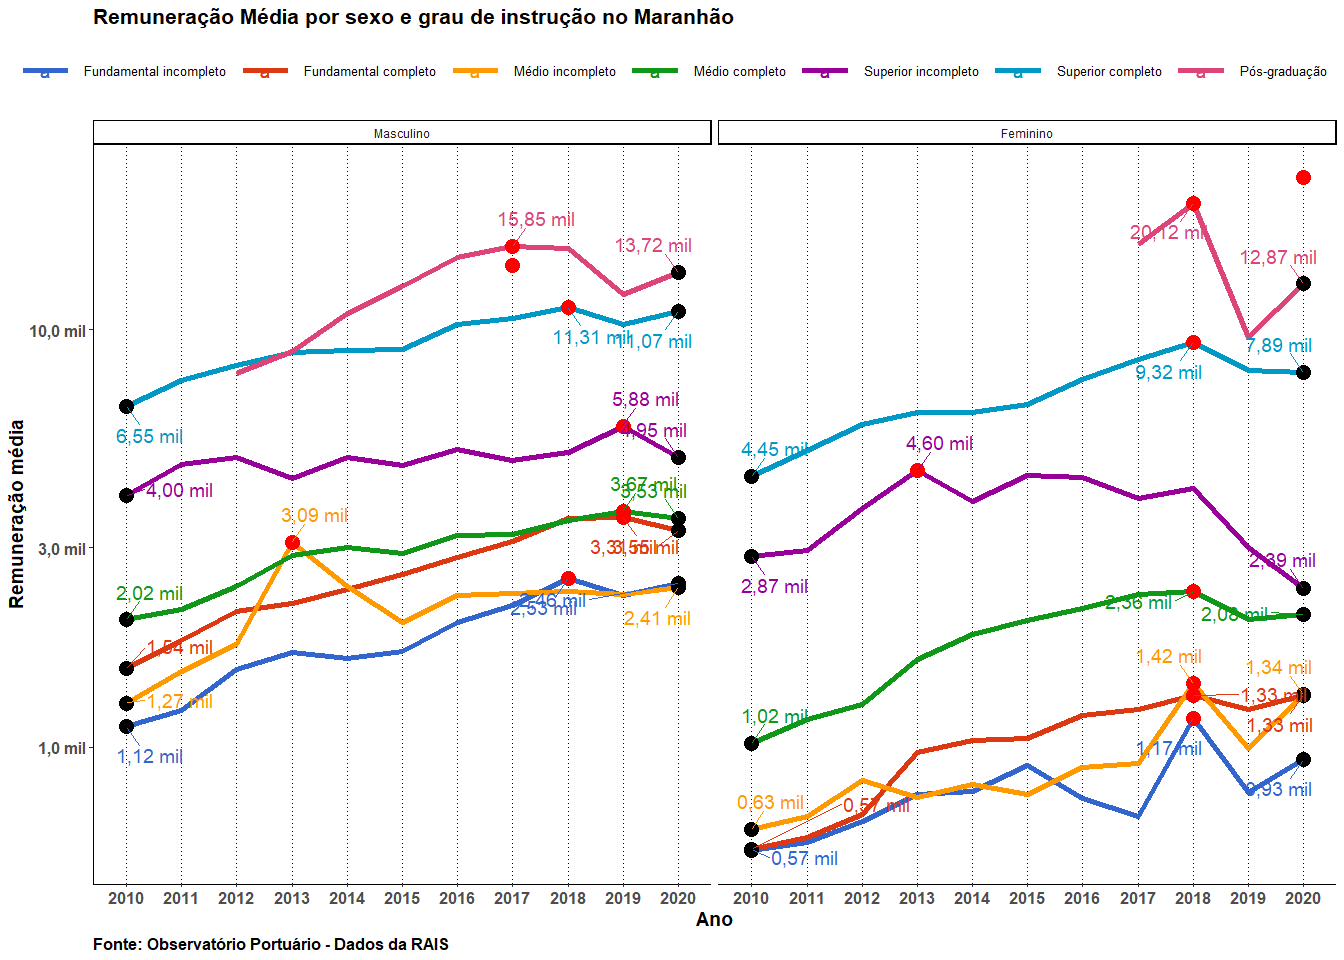
\includegraphics{mercado_trabalho_files/figure-latex/g_remun_escol_sexo.ma-1.pdf}

\hypertarget{rauxe7a-ou-cor-do-trabalhador-portuuxe1rio-e-aquaviuxe1rio}{%
\paragraph{Raça ou cor do Trabalhador Portuário e
Aquaviário}\label{rauxe7a-ou-cor-do-trabalhador-portuuxe1rio-e-aquaviuxe1rio}}

O perfil racial dos profissionais pode ser observado no gráfico a
seguir\footnote{Como há uma discrepância da quantidade de vínculos das
  categorias de \textbf{raça ou cor} quando comparadas por
  \textbf{sexo}, optou-se pela \textbf{escala logarítmica} no lugar da
  escala aritimética (escala habitual nos gráficos) para representar os
  dados quantidade de vínculos (\textbf{eixo y}) , pois a logarítmica
  permite, no caso do gráfico abaixo, uma visualização das tendências
  das quantidades de vínculos por cada raça ou cor ao longo dos anos
  analisados.}. Nota-se o predomínio de pardos e brancos, tanto entre os
homens como entre as mulheres.

Destaca-se ainda o alto registro da ausência de identificação racial nos
dados, o que é pauta para as ações de sensibilização dos profissionais
de gestão com pessoas e alinhado às ações de Governança Social. O
correto preenchimento dos dados pode auxiliar políticas de inclusão,
qualificação e diversidade mais assertivas.

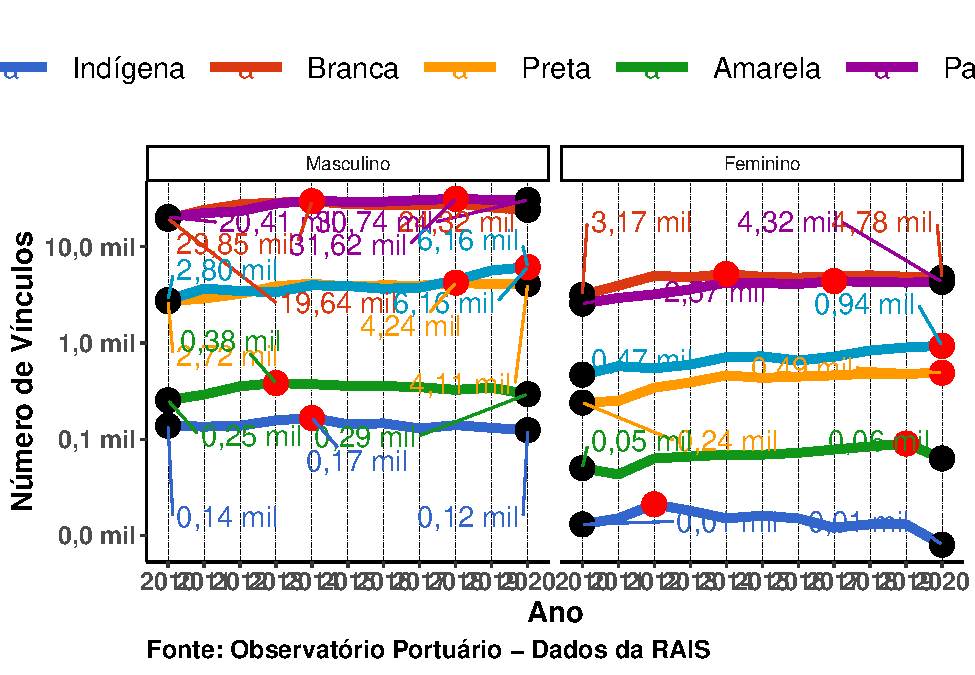
\includegraphics{mercado_trabalho_files/figure-latex/g_operacao_raca_sexo-1.pdf}

Apesar da destacada participação de pardos, a remuneração média desses
profissionais em 2020 era inferior a dos brancos. Nota-se que homens e
mulheres brancos tiveram a renda constante e crescente na série,
mantendo a assimetria em relação aos pretos e pardos.

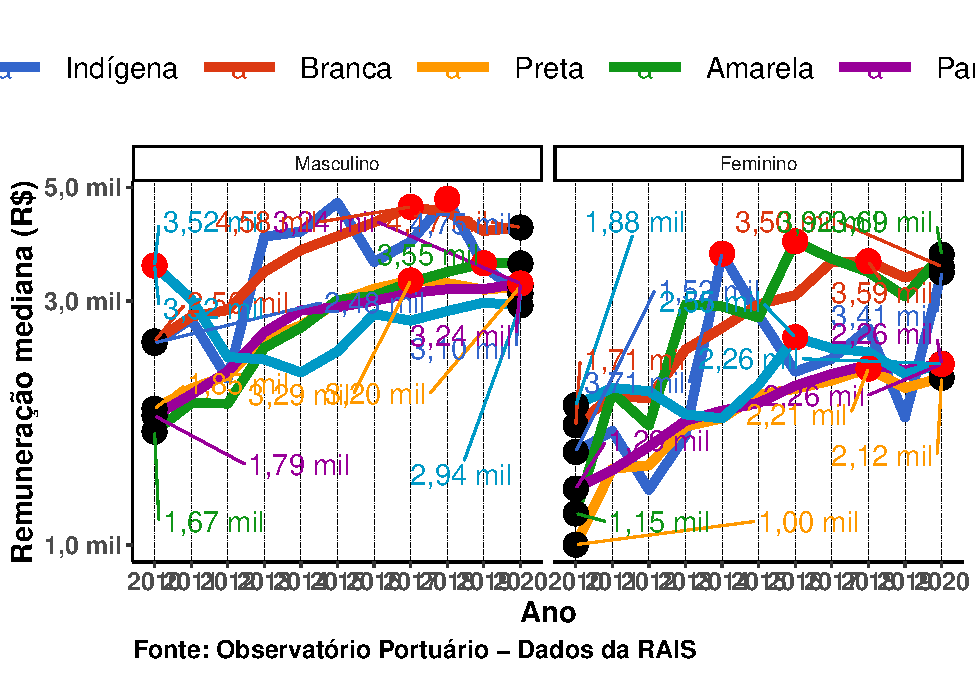
\includegraphics{mercado_trabalho_files/figure-latex/g_operacao_remuneracao _mediana_raca_sexo-1.pdf}

No Maranhão, os profissionais identificados como pardos predominam,
sendo seguidos pelos brancos e pretos entre os homens e mulheres.

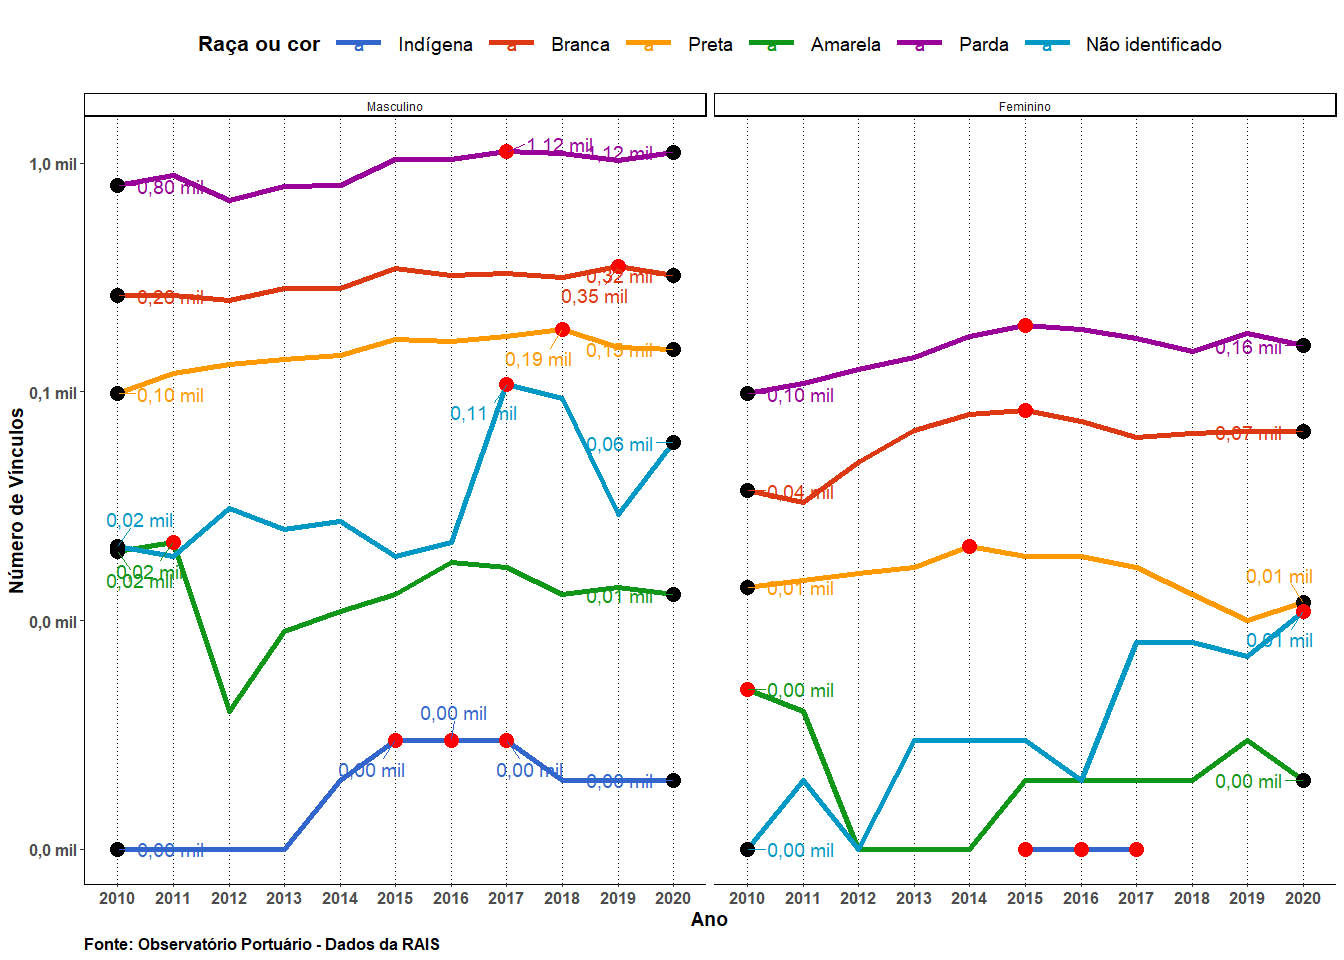
\includegraphics{mercado_trabalho_files/figure-latex/g_operacao_raca_sexo.ma-1.pdf}

A renda dos trabalhadores por cor ou raça no Maranhão, por sua vez,
evidencia que os autodeclarados amarelos se destacam entre os homens,
com remuneração mediana acima das demais (amarelos, de acordo com o
IBGE, são aqueles que se declaram de origem asiática: japoneses,
coreanos e chineses).

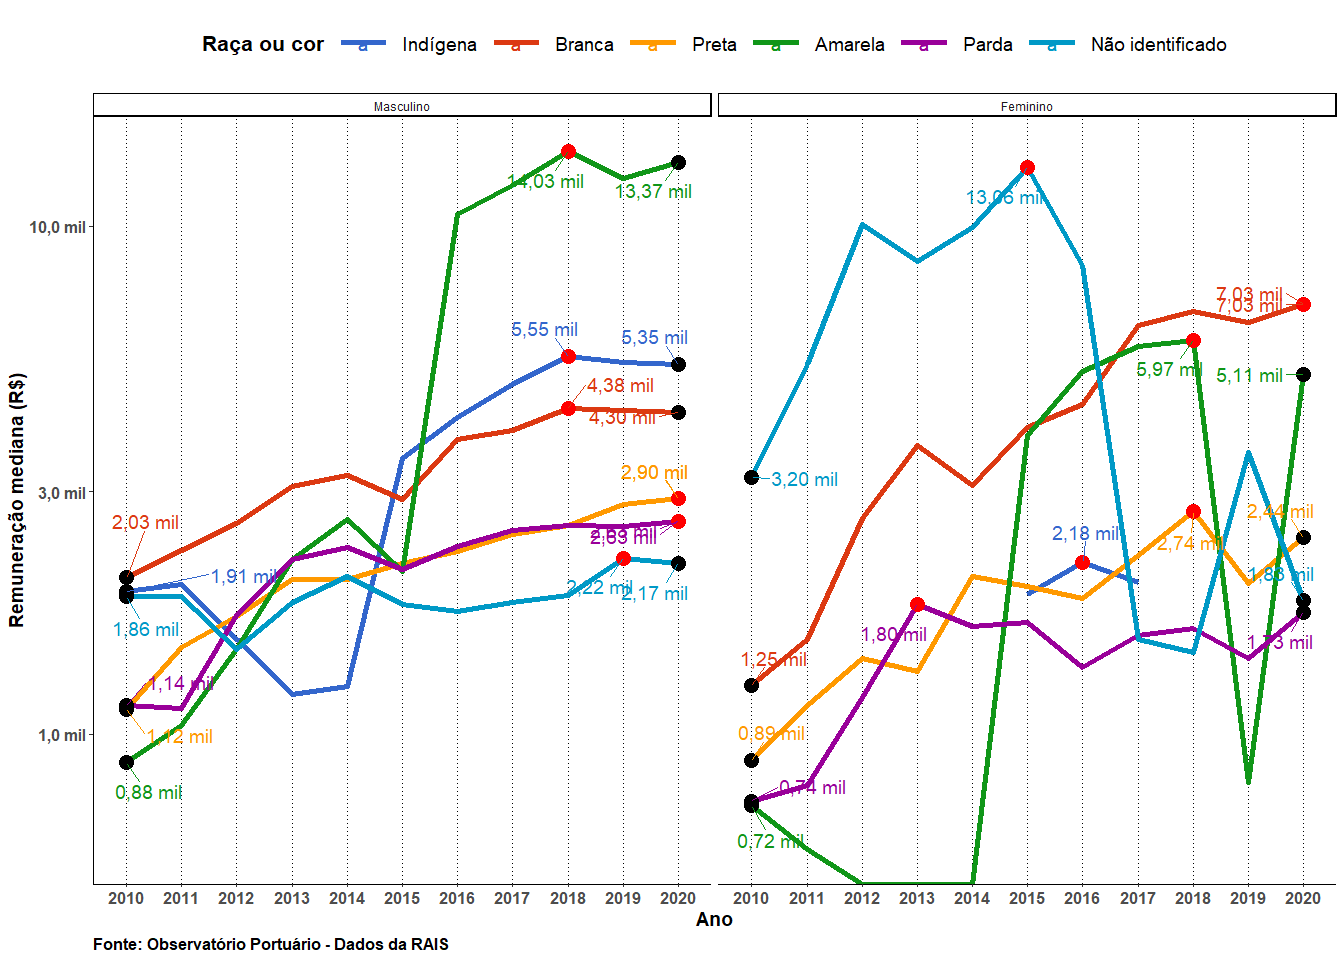
\includegraphics{mercado_trabalho_files/figure-latex/g_operacao_remuneracao _mediana_raca_sexo.ma-1.pdf}

\hypertarget{ocupauxe7uxf5es-dos-trabalhadores-portuuxe1rios-e-aquaviuxe1rios}{%
\subsection{Ocupações dos Trabalhadores Portuários e
Aquaviários}\label{ocupauxe7uxf5es-dos-trabalhadores-portuuxe1rios-e-aquaviuxe1rios}}

As ocupações com maior participação no setor estão no gráfico a seguir,
bem como a remuneração média respectiva.

Verifica-se que os profissionais \emph{Marinheiros de Convés (martítimo
e fluvial)} representam o maior contingente de profisisionais ao longo
do período analisado, embora com tendência decrescente e em número
inferior ao registrado em 2010.

Por usa vez, os Assistentes Administrativos mantiveram uma estabilidade
no número de vínculos, registrando cerca de 3.500 profissionais em 2020.

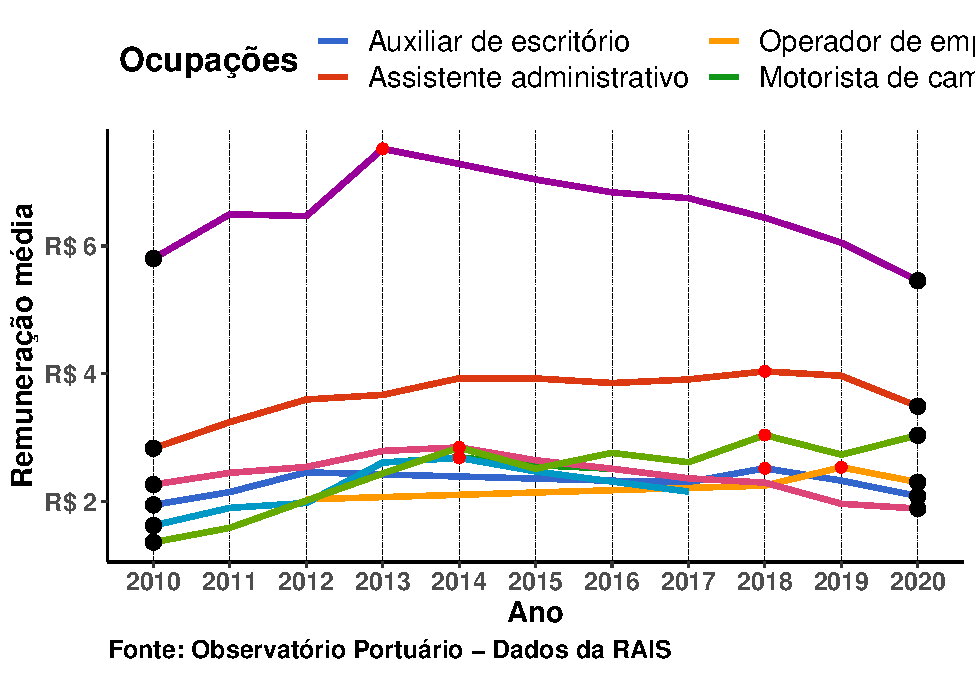
\includegraphics{mercado_trabalho_files/figure-latex/g_operacao_ocupacao-1.pdf}

\hypertarget{remunerauxe7uxe3o-dos-trabalhadores-nos-estados}{%
\subsection{Remuneração dos Trabalhadores nos
Estados}\label{remunerauxe7uxe3o-dos-trabalhadores-nos-estados}}

Verifica-se que a remuneração mediana dos trabalhadores portuários e
aguaviários varia conforme o estado da federação. O Rio de Janeiro é o
estado com a maior remuneração no período analisado, com o registro de
R\$ 8.535 em 2020. O Espírito Santo aparece em segundo lugar, com R\$
6.012.

O estado do Maranhão teve uma evolução signifitiva no valor da
remuneração mediana: saltou de R\$ 2.090 em 2010 para R\$ 4.765 em 2020.

\includegraphics{mercado_trabalho_files/figure-latex/g_operacao_estado_rem-1.pdf}

\hypertarget{remunerauxe7uxe3o-dos-trabalhadores-nos-municuxedpios}{%
\subsection{Remuneração dos Trabalhadores nos
municípios}\label{remunerauxe7uxe3o-dos-trabalhadores-nos-municuxedpios}}

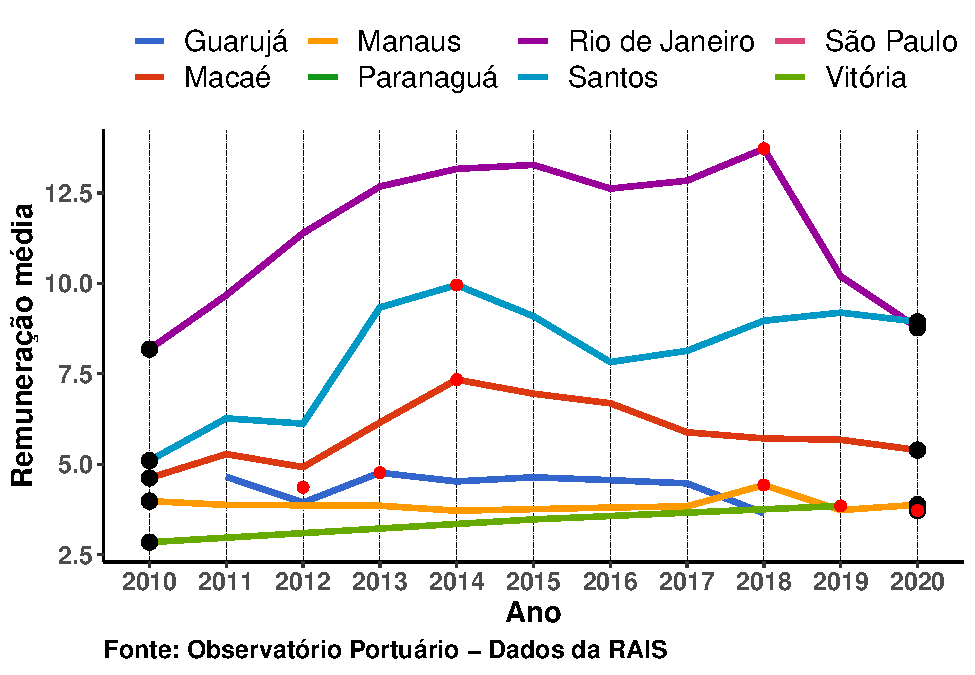
\includegraphics{mercado_trabalho_files/figure-latex/g_operacao_municipio-1.pdf}

\hypertarget{trabalhadores-da-gestuxe3o-e-operauxe7uxe3o-portuuxe1ria}{%
\section{Trabalhadores da Gestão e Operação
Portuária}\label{trabalhadores-da-gestuxe3o-e-operauxe7uxe3o-portuuxe1ria}}

O Brasil apresentou 52.469 vínculos de trabalho para a o setor
\textbf{portuário} e \textbf{aquaviário}. Em 2018, ano com a maior
quantidade de vínculos da série, foram 79.967 vínculos. Em 2020, último
ano da série histórica, foram 76.354 São Paulo e Rio de Janeiro
permanceram na primeira e segunda coloção durante toda a série. Em 2020,
por exempo, \textbf{Rio de Janeiro} possuía 22.731 vínculos
empregatícios e \textbf{São Paulo}, possuía cerca de 22.731. Por outro
lado, o estado do \textbf{Maranhão} possuía 1.924 vínculos no mesmo ano.

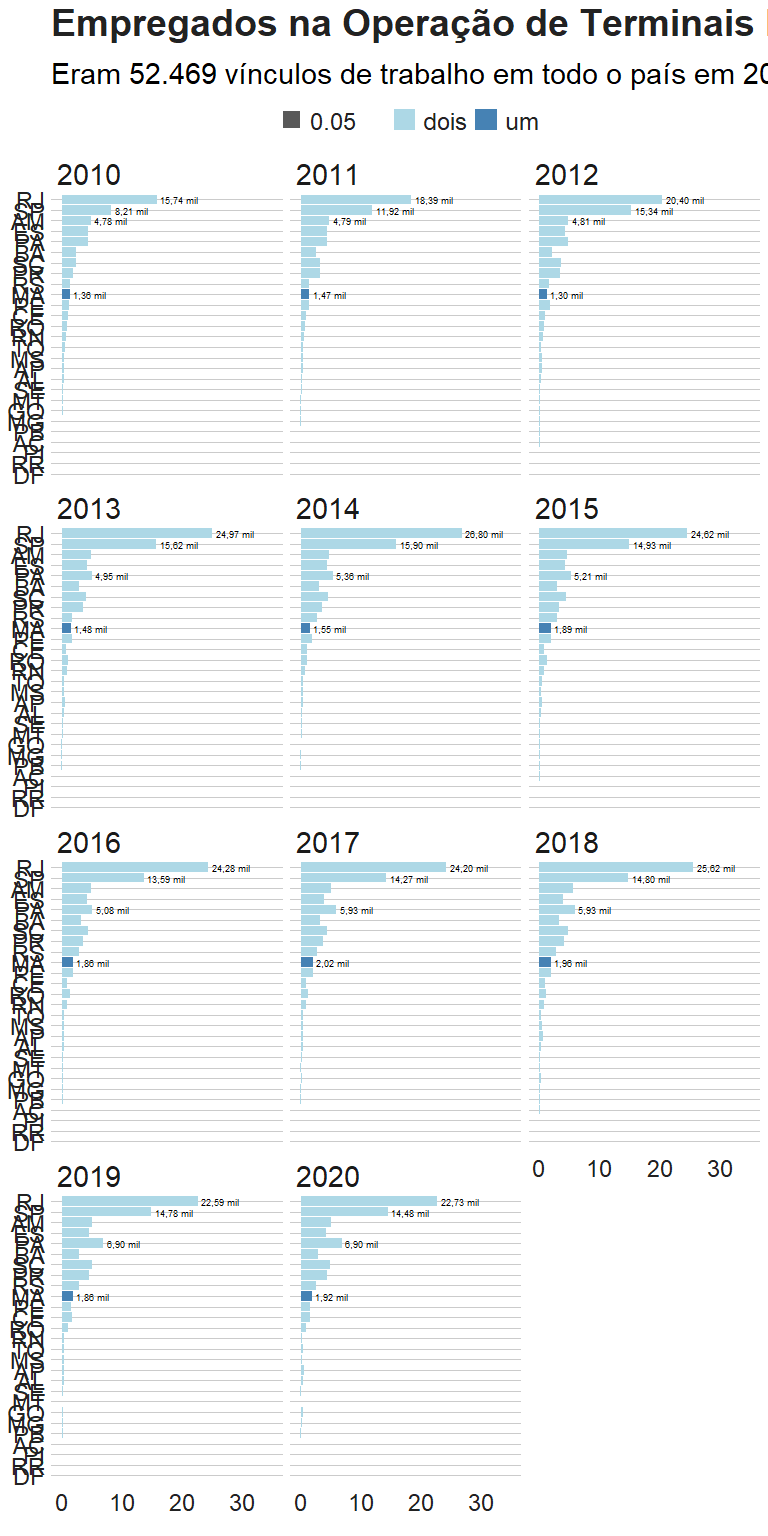
\includegraphics{mercado_trabalho_files/figure-latex/r g_operacao_uf-1.pdf}

\hypertarget{metodologia}{%
\section{Metodologia}\label{metodologia}}

Os dados apresentados neste relatório são originários da Relação Anual
de Informações Sociais (RAIS).

A RAIS é um registro administrativo que as organizações públicas e
privadas são obrigadas a enviar ao Ministério da Economia anualmente.
Seus dados, assim, abarcam estabelecimentos formais e permitem
identificar o estoque de vínculos formais de emprego (estatutários e
celetistas).

Este relatório apresenta os dados em uma perspectiva longitudinal:
apresenta os dados de 2010 a 2020.

O recorte dos dados sobre o trabalho portuário e aquaviário foi
realizado a partir da Classificação Nacional de Atividades Econômicas
(CNAE).

A CNAE é a classificação oficialmente adotada pelo Sistema Estatístico
Nacional e pelos órgãos federais gestores de registros administrativos e
está organizada em ordem decrescente de agregação das informações:
Seções, Divisões, Grupos, Classes e Subclasses.

A partir dessa divisão é possível mapear as atividades com trabalho
portuário e aquaviário e, especificamente, de operações e gestão
portuária.

Na tabela estão detalhadas as informações da CNAE utilizadas:

\begin{table}

\caption{\label{tab:tabela1}<center>Subclasses da Classificação Nacional de Atividades Econômicas 2.0 usadas <br> Seção H: Transporte, Armazenagem e Correio</center>}
\centering
\begin{tabular}[t]{>{}lllll}
\toprule
Seção & Divisão & Grupo & Classe & Subclasse\\
\midrule
 &  &  &  & Administração da infra-estrutura portuária\\
\cmidrule{5-5}
 & \multirow[t]{-2}{*}{\raggedright\arraybackslash ARMAZENAMENTO E ATIVIDADES AUXILIARES DOS TRANSPORTES} & \multirow[t]{-2}{*}{\raggedright\arraybackslash Atividades auxiliares dos transportes aquaviários} & \multirow[t]{-2}{*}{\raggedright\arraybackslash Gestão de portos e terminais} & Operações de terminais\\
\cmidrule{2-5}
 &  &  &  & Navegação de apoio marítimo\\
\cmidrule{5-5}
 &  & \multirow[t]{-2}{*}{\raggedright\arraybackslash Navegação de apoio} & \multirow[t]{-2}{*}{\raggedright\arraybackslash Navegação de apoio} & Navegação de apoio portuário\\
\cmidrule{3-5}
 &  &  &  & Transporte por navegação de travessia, intermunicipal\\
\cmidrule{5-5}
 &  &  & \multirow[t]{-2}{*}{\raggedright\arraybackslash Transporte por navegação de travessia} & Transporte por navegação de travessia, municipal\\
\cmidrule{4-5}
 &  &  &  & Outros transportes aquaviários não especificados anteriormente\\
\cmidrule{5-5}
 &  & \multirow[t]{-4}{*}{\raggedright\arraybackslash Outros transportes aquaviários} & \multirow[t]{-2}{*}{\raggedright\arraybackslash Transportes aquaviários não especificados anteriormente} & Transporte aquaviário para passeios turísticos\\
\cmidrule{3-5}
 &  &  &  & Transporte marítimo de cabotagem - Carga\\
\cmidrule{5-5}
 &  & \multirow[t]{-2}{*}{\raggedright\arraybackslash Transporte marítimo de cabotagem e longo curso} & \multirow[t]{-2}{*}{\raggedright\arraybackslash Transporte marítimo de cabotagem} & Transporte marítimo de cabotagem - passageiros\\
\cmidrule{3-5}
 &  &  &  & Transporte por navegação interior de carga, intermunicipal, interestadual e internacional, exceto travessia\\
\cmidrule{5-5}
 &  &  & \multirow[t]{-2}{*}{\raggedright\arraybackslash Transporte por navegação interior de carga} & Transporte por navegação interior de carga, municipal, exceto travessia\\
\cmidrule{4-5}
 &  &  &  & Transporte por navegação interior de passageiros em linhas regulares, intermunicipal, interestadual e internacional, exceto travessia\\
\cmidrule{5-5}
\multirow[t]{-14}{*}{\raggedright\arraybackslash \textbf{H}} & \multirow[t]{-12}{*}{\raggedright\arraybackslash TRANSPORTE AQUAVIÁRIO} & \multirow[t]{-4}{*}{\raggedright\arraybackslash Transporte por navegação interior} & \multirow[t]{-2}{*}{\raggedright\arraybackslash Transporte por navegação interior de passageiros em linhas regulares} & Transporte por navegação interior de passageiros em linhas regulares, municipal, exceto travessia\\
\bottomrule
\multicolumn{5}{l}{\rule{0pt}{1em}\textit{Note: } makecell[l]{Observatório Portuário \Dados: IBGE - CNAE}}\\
\end{tabular}
\end{table}

\end{document}
